%
% chapter.tex -- Beschreibung des Inhaltes
%
% (c) 2021 Prof Dr Andreas Müller, Hochschule Rapperswil
%
% !TeX spellcheck = de_CH
\chapter{Exponentialfunktion und Exponentialgleichungen
\label{buch:chapter:exponential}}
\lhead{Exponentialfunktion und Exponentialgleichungen}
\rhead{}

%
% zins.tex
%
% (c) 2021 Prof Dr Andreas Müller, OST Ostscheizer Fachhochschule
%
\section{Exponentialfunktion als Grenzwert
\label{buch:exponential:section:grenzwert}}
\rhead{Exponentialfunktion als Grenzwert}

\subsection{Permanente Verzinsung}

\subsection{Eulerscher Grenzwert}


%
% log.tex
%
% (c) 2021 Prof Dr Andreas Müller, OST Ostschweizer Fachhochschule
%
\section{Logarithmen
\label{buch:exponential:section:logarithmen}}
Heutezutage wird die Logarithmusfunktion als die Umkehrfunktion
der Exponentialfunktion definiert.
Ihren Ursprung hat sie jedoch im Bemühen, eine Methode zur Vereinfachung
der numerischen Rechnung zu finden.
In diesem Abschnitt soll die Geschichte kurz nachgezeichnet werden.

\subsection{Multiplikation}
Die Schwierigkeit besteht vor allem darin, dass Multiplikationen
sehr viel aufwendiger sind als Additionen.
So braucht man für die Addition zweier $n$-stelliger Zahlen
genau $n$ Additionen einstelliger Zahlen mit Übertrag.
Für die Multiplikation sind zunächst $n^2$ einstellige Multiplikationen
gefolgt von $n(n-1)$ Additionen einstelliger Zahlen mit Übertrag notwenig,
um einen Faktor mit jeder Stelle des anderen zu multiplizieren.
Anschliessend müssen dann $(n-1)^2$ einstellige Multiplikationen
gefolgt von einstelligen Additionen mit Übertrag ausgeführt werden,
um die Summe zu bilden.
Der Aufwand für eine Multiplikation wächst also quadratisch mit
der Genauigkeit, während der Aufwand für die addition nur linear
anwächst.

Eine gebräuchlich Methode war die Verwendung der trigonometrischen
Identität
\begin{align*}
\sin(\alpha)\sin(\beta)
&=
\frac12
\cos(\alpha-\beta)
-
\frac12
\cos(\alpha+\beta).
\intertext{Dies kann mit einer Tabelle nur der Sinus-Werte durchgeführt
werden, indem man verwendet, dass $\sin x = \cos(90^\circ-x)$.
Dies führt auf die Identität }
\sin(\alpha)\sin(\beta)
&=
\frac12\bigl(\sin(90^\circ-\alpha+\beta)
-
\sin(90^\circ-\alpha-\beta)\bigr)
\end{align*}
Die Multiplikation der Zahlen $\sin\alpha$ und $\sin\beta$ verlangt
daher nur zwei Konsultationen der Sinus-Tabelle, um die Winkel
$\alpha$ und $\beta$ zu bestimmen, zwei Additionen zur Berechnung
von 
$90^\circ-\alpha+\beta$
und
$90^\circ-\alpha-\beta$,
zwei Konsultationen der Sinus-Tabelle gefolgt von einer Addition
und einer
Halbierungsoperationen, die sich ähnlich effizient wie Additionen
durchführen lässt.
Der Aufwand dieser Art der Durchführung der Multplikation ist also
gleich gross wie $4$ Additionen und $4$ Tabellenkonsultationen.

\begin{beispiel}
In Abschnitt~\ref{buch:trigo:subsection:tabelle} ist beschrieben, wie
schon im Altertum Tabellen für Sinus-Werte aufgestellt werden konnten.
Mit der Tabelle~\ref{buch:trigo:table:sinus} kann man zum Beispiel die
folgende Multiplikation durchführen.
Gesucht ist das Produkt der Zahlen $x=0.51503807$ und $y=0.80901169$.
Die Berechnung läuft wie folgt ab:
\begin{align*}
x&=0.80901169&
&\Rightarrow&\sin\alpha  &=x&
&\Rightarrow&{\color{red}\alpha}&\approx {\color{red}54^\circ}
\\
y&=0.51503807&
&\Rightarrow&\sin\beta   &=y&
&\Rightarrow&{\color{red}\beta}&\approx {\color{red}31^\circ}
\\
 &          &
&           &{\color{red}\sin\delta_1}&={\color{red}0.92050485}&
&\Leftarrow &{\color{blue}\delta_1}&=90^\circ-\alpha+\beta={\color{blue}67}
\\
 &          &
&           &{\color{red}\sin\delta_2}&={\color{red}0.08715574}&
&\Leftarrow &{\color{blue}\delta_2}&=90^\circ-\alpha-\beta={\color{blue}5}
\\
 &&
 &          &{\color{blue}\sin\delta_1+\sin\delta_2}&={\color{blue}0.83334911}
\\
xy&=0.41667455&
 &\Leftarrow&\frac12(\sin\delta_1+\sin\delta_2)&={\color{darkgreen}0.41667455}
\end{align*}
Die roten Zahlen sind Resultate von Tabellenkonsultationen, die blauen
ergeben sich durch Additionen, grün ist die Halbierungsoperation.
Alle acht Stellen des Resultates sind korrekt.
\end{beispiel}

Das Verfahren funktioniert also, hat aber eine ganze Reihe von Nachteilen:
\begin{enumerate}
\item
Die Zahl der Operationen ist ziemlich gross.
Immerhin sind vier Tabellenkonsultationen nötig, drei Additionen und die
Halbierungsoperation.
\item
Es funktioniert nur für Zahlen zwischen $0$ und $1$.
Für Zahlen ausserhalb dieses Intervalls ist es die Aufgabe des
Anwenders, eine Skalierung vorzunehmen und sie später bei der Angabe
des Resultates wieder einfliessen zu lassen.
Das Quadrat von $2$ kann berechnet werden als
\(2^2 = 100 \cdot 0.2\cdot 0.2\), was mit dem Winkel
$\alpha=\beta=11.537^\circ$ möglich ist. 
Das Resultat der Multiplikation nach obigem Verfahren ist dann 
\[
\frac12\bigl(
\sin(90^\circ-\alpha+\beta)
-
\sin(90^\circ-\alpha-\beta)
\bigr)
=
\frac12\bigl(
1-
\sin 66.926^\circ
\bigr)
=
\frac12( 1-0.9200)
=
\frac12\cdot 0.08=0.04,
\]
woraus sich dann das Quadrat von $2$ als
$2^2 = 100\cdot 0.2^2 = 100\cdot 0.04 = 4$
ergibt.
Dieser Nachteil gilt allerdings auch für Rechenverfahren mit Logarithmen
oder mit einem Rechenschieber, bei dem ebenfalls nur die Mantisse
berechnet wird, der Anwender ist selbst für die Bestimmung des Exponenten
verantwortlich.
\item
Es kann vorkommen, dass die Winkel $90^\circ-\alpha+\beta$
und $90^\circ-\alpha-\beta$ nicht im Intervall zwischen $0$ und $90^\circ$
liegen.
In diesem Fall ist eine zusätzliche Reduktion des Winkels nötig.
Falls der Winkel negativ ist, muss in den folgenden Schritt zusätzlich
das Vorzeichen berücksichtigt werden.
\end{enumerate}


\subsection{Die Erfindung der Logarithmen}
Die Lösung des Problems ist die Verwendung von Exponentialfunktionen 
anstelle von trigonometrischen Funktionen.
Um das Produkt von zwei Zahlen $x$ und $y$ zu bestimmen, müssen erst
die Exponenten $\xi$ und $\eta$ bestimmt werden, für die $x=b^\xi$
$y=b^\eta$ ist.
Das Produkt ist dann $xy = b^{\xi+\eta}$, es muss also die Summe
$\xi+\eta$ berechnet werden und aus einer Tabelle der Funktion
$b^\bullet$ kann dann das Produkt abgelesen werden.
Der Wert der Basis $b$ ist dabei noch frei und wurde auch von
den Erfindern der Logarithmen verschieden angegangen.

\subsubsection{Die arithmetischen Progresstabulen von Jost Bürgi}
\begin{figure}
\centering
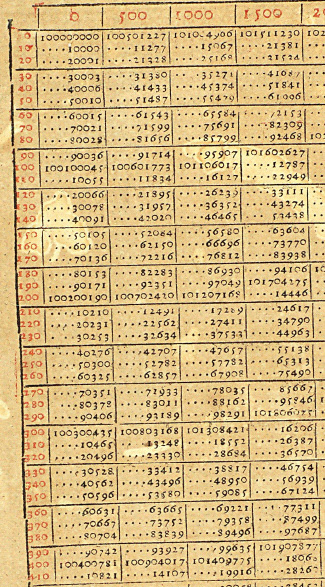
\includegraphics{chapters/020-exponential/images/Log_Calc-Figure7.jpeg}
\caption{Ausschnitt aus der ersten Seite von Jost Bürgis Tabelle der
Potenzen von $1.0001$
\label{buch:exponential:log:fig:buergi1}}
\end{figure}
\begin{figure}
\centering
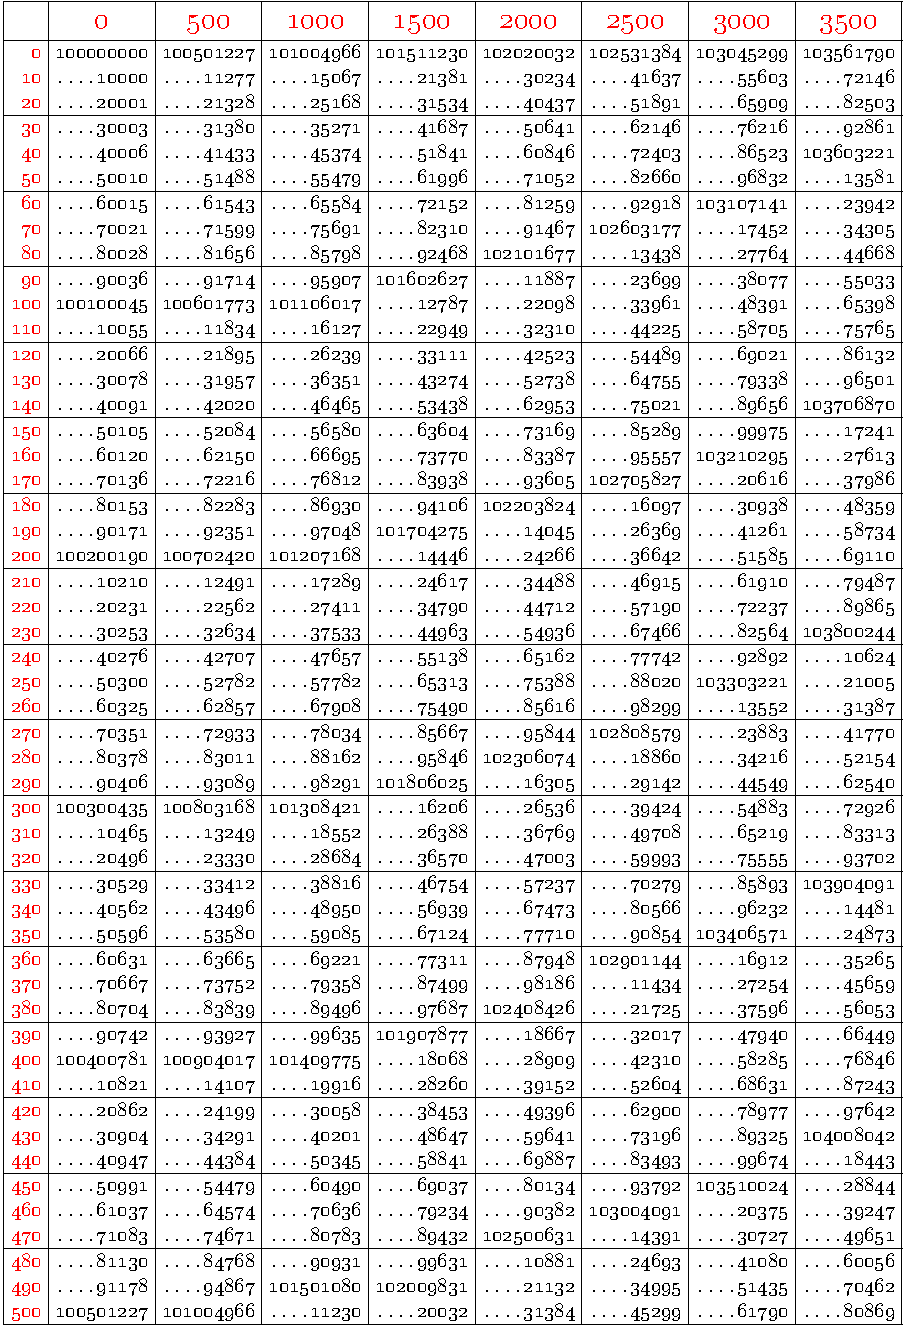
\includegraphics[width=0.92\textwidth]{chapters/020-exponential/images/buergiausschnitt.pdf}
\caption{Rekonstruktion der ersten Seite von Bürgis Tabelle aus
\cite{buch:hal}
\label{buch:exponential:log:fig:buergi2}}
\end{figure}
Der 1552 in Lichtensteig geborene schweizer Uhrmacher und Mathematiker
hat in seinem Werk
{\em Arithmetische und geometrische Progress Tabulen sambt gründlichem 
unterricht, wie solche nützlich in allerley Rechnungen zugebrauchen
und verstanden werden soll}, welches 1620 in Prag erschien,
eine Tabelle aller Werte
\[
10^8\cdot\biggl(1+\frac{1}{10000}\biggr)^n
=
10^8 \biggl(\biggl(1+\frac{1}{10000}\biggr)^{10000}\biggr)^{n\cdot10^{-4}}
\]
für $n=0$ bis $n=23027$.
Die Abbildung~\ref{buch:exponential:log:fig:buergi1}
zeigt, einen Ausschnitt aus der ersten Seite von Bürgis Tabelle.
Die mit 10 multiplizierten Exponenten $n$ sind durchwegs als
{\color{red}rote} Zahlen dargestellt.
In jeder Spalten stehen 40 aufeinanderfolgende Werte, von Spalte
zu Spalten nimmt der Wert von $n$ um 500 zu.
Abbildung~\ref{buch:exponential:log:fig:buergi2} zeigt eine Rekonstruktion
der ersten Seite.

Um mit der Bürgischen Tafel eine Multiplikation durchzuführen,
hat man also unter den schwarzen Zahlen Werte gesucht,
der möglichst nahe an den gegebenen Faktoren sind.
Dabei konnte die Genauigkeit noch gesteigert werden, indem zwischen
aufeinanderfolgenden Werten interpoliert wurde.
Die zugehörigen roten Zahlen wurden dann addiert und mit Hilfe der
Tabelle wieder die schwarzen Zahlen ermittelt.

\begin{beispiel}
Die erste Seite \ref{buch:exponential:log:fig:buergi2} der Bürgischen
Tabelle umfasst natürlich nur einen sehr kleine Teil des ganzen Werkes,
trotzdem kann man daran den Gang der Rechnung illustrieren.
Um die beiden schwarzen Zahlen $x=1.0023$ und $y=1.0017$ miteinander
zu multiplizieren, sucht man die zugehörigen roten Zahlen in
der Tabelle
\[
\renewcommand{\arraycolsep}{2pt}
\begin{array}{rclcr}
            & &\text{schwarze Zahl}&&\text{{\color{red}rote Zahl}} \\
           x&=&1.0023      &\Rightarrow&{\color{red}2274}\\
           y&=&1.0017      &\Rightarrow&{\color{red}1686}\\
          xy&=&1.004039247 &\Leftarrow &{\color{red}3960}
%\text{exakt}&=&1.0040391   &           &
\end{array}
\]
Das exakte Result ist $xy=1.0040391$.
\end{beispiel}

Die roten Zahlen werden in heutiger Terminologie Logarithmen zur
Basis $b=1.0001$ im Wesentlichen genannt.
In der Tabelle werden die Werte von $b^n$ in Abhängigkeit von $n$
angegeben, es wurde also direkt die Exponentialfunktion $b^\bullet$
tabuliert.
In heutiger Sprechweise würde man dies als eine Antilogarithmentafel
bezeichnen.

\subsubsection{John Napier und die natürlichen Logarithmen}
Der schottische Mathematiker John Napier (1550--1617) hat ein
ausgeklügeltes Verfahren entwickelt, 
natürliche Logarithmen mit hoher Genauigkeit von mindestens sieben
Stellen zu berechnen.
Ausserdem hat er den Logarithmen ihren Namen gegeben.

Um die Genauigkeit von sieben Stellen zu erreichen, musste er von
einem Wert ausgehen, der nicht weiter als $10^{-7}$ von $1$ entfernt
ist.
Bürgi hat mit dem Wert $1+10^{-4}$ eine Genauigkeit von vier Stellen
erreicht, Napier startete seine Berechnung mit $1-10^{-7}$.
Er hat also eigentlich Logarithmen zur Basis $1/e$ bestimmt.

Hätte Napier jedoch einfach nur das Verfahren von Bürgi auf die um
den Faktor $10^3$ höhere Genauigkeit angewendet, hätte er auch $10^3$
mal mehr und somit über 23 Millionen Multiplikationen durchführen
müssen, im Laufe derer sich viel zu grosse Rundungsfehler akkumuliert
hätten.
Napier hat daher das gesamte Intervall in mehrer grössere Intervall
unterteilt, indem er mit statt nur den Faktor $a=1-10^{-7}=0.9999999$
auch noch geometrische Folgen mit den Faktoren $b=1-10^{-5}=0.99999$ und
$c=1-5\cdot10^{-4}=0.9995$ verwendet hat.
Mit 4604 Gliedern der Folge $c^k$ konnte er tatsächlich das ganze
Intervall zwischen $0.1$ und $1$ geometrisch unterteilen.
Innerhalb jedes Teilintervalls kann dann eine Unterteilung mit
50 Gliedern der Folge $b^k$ aufteilen.
Und schliesslich liefern 100 Gleider der Folge $a^k$ eine geometrische
Unterteilung in jedes dieser Intervalle.
Auf diese Art kann erreicht werden, dass jeder Wert mit höchstens 4755
Multiplikationen und damit ohne Kompromittierung der Genauigkeit durch
Rundungsfehler berechnet werden kann.

Das Interpolationsverfahren, welches Napier zur Bestimmung seiner 
Logarithmen entwickelt hat, hat auch die Entwicklung von Rechenschiebern
motiviert.

\subsubsection{Dekadische Logarithmen nach Henry Briggs}
Henry Briggs (1561--1630) hat die Bedeutung der Napierschen
Logarithmen sofort erkannt und vorgeschlagen, statt der Basis $e$
die Basis $10$ zu verwenden. 
Der Vorteil der Basis 10 ist, dass Zahlen mit der gleichen
Mantisse in Gleitkommadarstellung zur Basis 10 Logarithmen haben,
die sich nur im eine Ganzzahl unterschieden, die gleichzeitig der
Unterschied der Exponenten ist.
Dies macht die Verwendung einer Logarithmentabelle sehr viel
intuitiver.

Briggs hat ausserdem die numersiche Berechnung der Logarithmen 
weiterentwickelt und innerhalb von 7 Jahren 30000 Logarithmen mit
einer Genauigkeit von 14 Stellen berechnet.
Die Methoden von Bürgi und Napier gingen davon aus, das Intervall,
in dem die Logarithmen bestimmt werden sollen, durch Konstruktion
einer geometrischen Folge zu unterteilen.
Zum Beispiel hat Bürgi das Intervall von $1$ bis $10$ mit Hilfe von
23027 Multiplikationen von $1.0001$ zu unterteilen.
Briggs fragte sich daher, ob sich eine Unterteilung auch in weniger
Schritten erreichen liesse.

Welchen Faktor $a$ muss man nehmen, wenn man das Intervall von
$1$ bis $10$ geometrisch in zwei Teilintervalle unterteilen will.
Der Faktor $a$ muss $a^2=10$ erfüllen, also $a=\sqrt{10}$.
Somit haben wir in $\sqrt{10}$ einen Wert mit einem genau
bekannten Zehnerlogarithmus von $0.5$ gefunden.

Durch Iteration dieser Idee kann man durch $n$-faches
wiederholtes Wurzelziehen die Zahlen mit den bekannten
Logarithmen $2^{-n}$ bestimmen.
Durch Darstellung eines Logarithmus im Binärsystem kann
man dann die zugehörige Zahl durch nur so viele Multiplikationen
bestimmen, wie Einsen in der Binärdarstellung des Logarithmus
vorkommen.
Damit ist der Rechenaufwand für die Berechnung einzelner
Logarithmen sehr viel kleiner also in den Methoden von Bürgi
und Napier.

Die Briggssche Idee funktioniert besonders gut im Binärsystem,
wenn also Logarithmen für Zahlen zwischen $1$ und $2$ bestimmt
werden müssen.
Im Binärsystem ist Division durch $2$ besonders einfach, sie ist
einfach nur eine Verschiebung des Kommas.
Auch für die Berechnung der Quadratwurzel gibt es effiziente
binäre Algorithmen.









%
% lambertw.tex
%
% (c) 2021 Prof Dr Andreas Müller, OST Ostschweizer Fachhochschule
%
\section{Die Lambert $W$-Funktion
\label{buch:section:lambertw}}
\rhead{Lambert $W$-Funktion}
Exponentialgleichungen wie
\[
e^{2x}+2e^x-15=0
\]
können durch Substitution $y=e^x$ in eine algebraische Gleichung
umgeformt werden, die mit Wurzelfunktionen gelöst werden kann.
Eine solche Substitution ist nicht mehr möglich, wenn Produkte
der Unbekannten und der Exponentialfunktion, also $xe^x$ auftreten.
Die Lambert $W$-Funktion ermöglicht, die Lösungen solcher Gleichungen
darzustellen.

%
% Die Funktion xe^x
%
\subsection{Die Definition der Lambert $W$-Funktion
\label{buch:subsection:funktion-xexpx}}
\begin{figure}
\centering
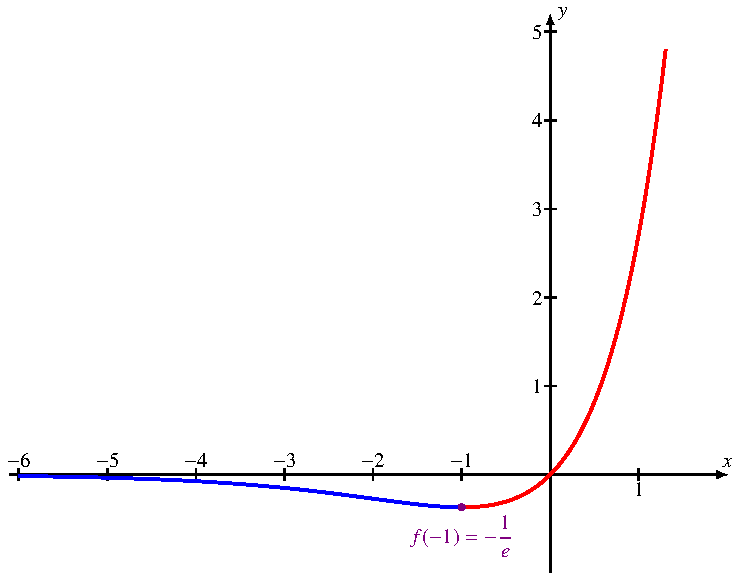
\includegraphics{chapters/020-exponential/images/xexpx.pdf}
\caption{Graph der Funktion $f\colon x\mapsto f(x)=xe^x$
\label{buch:lambert:graph}}
\end{figure}
Ein Graph der Funktion 
\[
f\colon \mathbb{R}\to\mathbb{R} : x\mapsto xe^x
\]
ist in Abbildung~\ref{buch:lambert:graph} dargestellt.
Die einzige Nullstelle ist bei $x=0$.
Die Funktion $f$ hat die Ableitung
$f'(x)=e^x + xe^x$,
an  der Stelle $x=0$ hat der Graph von $f(x)$ daher die Steigung $1$.

Die Ableitung verschwindet für
\[
0 = f'(x) = e^x(1+x)
\qquad\Rightarrow\qquad
x=-1,
\]
dort hat die Funktion $f$ den minimalen Wert $-1/e$.

Wegen des Minimums an der Stelle $x=-1$ ist die Funktion $f(x)$ nicht
umkehrbar.
Auf dem Teilintervall $I_{-1}=(-\infty,-1]$ ist $f$ streng
monoton fallend, auf dem Teilintervall $I_0=[-1,\infty)$ ist sie
streng monoton wachsen.
Die Einschränkung von $f$ auf diese beiden Intervalle ist also
invertierbar.

\begin{definition}
Die inverse Funktion der Funktion $[-1,\infty)\to[-1/e,\infty):x\mapsto xe^x=y$
heisst die Lambert $W$-Funktion, geschrieben $W(y)$ oder $W_0(y)$.
Die inverse Funktion der Funktion $(-\infty,-1)\to[-1/e,0)$ wird mit
$W_{-1}$ bezeichnet.
\end{definition}

\begin{figure}
\centering
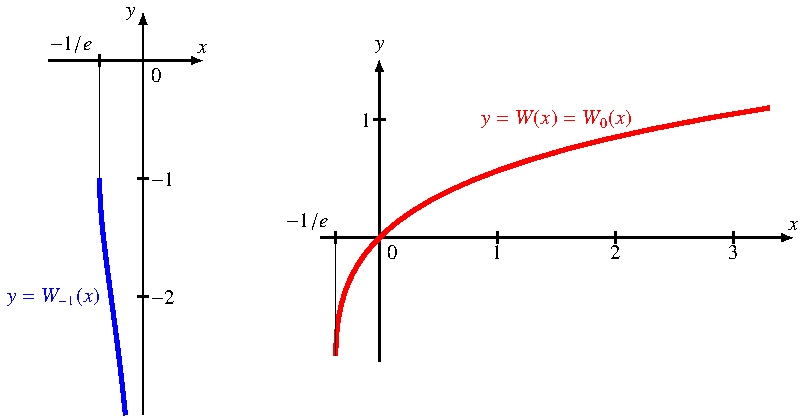
\includegraphics{chapters/020-exponential/images/w.pdf}
\caption{Graph der Funktionen $W_{-1}(x)$ (links) und $W_0(x)$ (rechts)
\label{buch:lambert:wgraph}}
\end{figure}
Die beiden Funktion $W_0(x)$ und $W_{-1}(x)$ sind in
Abbildung~\ref{buch:lambert:wgraph} dargestellt.
Beide Funktionen sind streng monoton und haben unendlich grosse Steigung
an der Stelle $x=-1/e$.

Da die $W$-Funktionen Umkehrfunktionen der Funktion $f(x)=xe^x$ sind,
erfüllen sie
\[
W(x) e^{W(x)} = x.
\]

\subsubsection{Ableitung der Funktionen $W(x)$ und $W_{-1}(x)$}
Die Umkehrfunktion $f^{-1}(y)$ einer Funktion $f(x)$ erfüllt
\(
f^{-1}(f(x)) = x.
\)
Ableitung nach $x$ ergibt mit der Kettenregel
\[
\frac{df^{-1}(y)}{dy}\bigg|_{y=f(x)} \frac{df}{dx} = 0
\qquad\Rightarrow\qquad
(f^{-1})'(y) = \frac{1}{f'(x)}.
\]
Für die $W$-Funktion, also für $W(y)=x$ oder $y=f(x)=xe^x$ bedeutet dies
\[
W'(y)
=
\frac{1}{f'(x)}
=
\frac{1}{f'(W(y))}.
\]
Die Ableitung von $f$ an der Stelle $W(y)$ ist
\[
f'(W(y))
=
(1+x)e^x
=
(1+W(y))e^{W(y)}.
\]
Die Exponentialfunktion von $W(y)$ ist
\[
e^{W(y)} = \frac{y}{W(y)},
\]
womit die Ableitung der $W$-Funktion
\begin{equation}
W'(y)
=
\frac{W(y)}{y}\cdot \frac{1}{1+W(y)}
=
\frac{W(y)}{y(1+W(y))}
\label{buch:lambert:eqn:ableitung}
\end{equation}
wird.

Aus der ersten Ableitung kann jetzt mit Hilfe der Quotientenregel
auch jede höhere Ableitung berechnet werden.
Die zweite Ableitung ist
\begin{align*}
\frac{d^2}{dy^2}W(y)
&=
\frac{d}{dy}W'(y)
=
\frac{d}{dy}\frac{W(y)}{y(1+W(y))}
\\
&=
\frac{
W'(y)y(1+W(y)) - W(y)\bigl(1+W(y)+yW'(y)\bigr)
}{
y^2(1+W(y))^2
}
\\
&=
\frac{
W'(y)y - W(y)(1+W(y))
}{
y^2(1+W(y))^2
}.
\intertext{Die Ableitung $W'(y)$ kann jetzt durch
\eqref{buch:lambert:eqn:ableitung} ersetzt werden, dies ergibt}
&=
\frac{
\displaystyle
\frac{W(y)}{y(1+W(y))}y - W(y)(1+W(y))
}{
y^2(1+W(y))^2
}
\\
&=
\frac{
W(y) - W(y)(1+W(y))^2
}{
y^2(1+W(y))^3
}
\\
&=
\frac{
-2W(y)^2-W(y)^3
}{
y^2(1+W(y))^3
}
\\
&=
-
\frac{
W(y)^2
}{
y^2(1+W(y))^3
}
(W(y)+2).
\end{align*}
Nach dem selben Muster können beliebig hohe Ableitungen von $W(y)$ durch
$W(y)$ ausgedrückt werden.
Zum Beispiel findet man nach einiger Rechnung für die dritte und vierte
Ableitung der $W$-Funktion die Ausdrücke
\begin{align*}
W'''(x)
&=
\phantom{-}
\frac{W(y)^3}{y^3(1+W(y))^4}\cdot (2W(y)^2 + 8W(y)+9)
\\
W''''(x)
&=
-\frac{W(y)^4}{y^4(1+W(y))^5}\cdot (6W(y)^3 + 36W(y)^2 + 79W(y) + 64).
\end{align*}
Mit etwas zusätzlicher Arbeit kann man für die $n$-te Ableitung
\[
\frac{d^n}{dy^n} W(y)
=
\frac{(-1)^{n+1}W(y)^n}{y^n(1+W(y))^{n+1}} \cdot P_n(W(y)),
\]
wobei die Polynome $P_n(t)$ die Rekursionsgleichung
\[
P_{n+1}(t)
=
(nt+3n-1)\cdot P_n(t) - (t+1)\cdot P'_n(t)
\]
mit $P_1(t)=1$.

\subsubsection{Differentialgleichung und Stammfunktion}
Die Ableitungsformel \eqref{buch:lambert:eqn:ableitung} bedeutet auch,
dass die $W$-Funktion eine Lösung der Differentialgleichung
\[
\frac{dW}{dz}
=
\frac{W}{z(1+W)}
\qquad
\text{mit Anfangsbedingung}
\qquad
W(0) = 1
\]
ist.
Diese Gleichung kann separiert werden in
\[
(1+W)\frac{dW}{W} = \frac{dz}{z}.
\]

Eine Stammfunktion
\[
F(y)
=
\int W(y)\,dy
\]
von $W$ kann mit der Substition $w=W(y)$ gefunden
werden, also $we^w=y$.
Die Ableitung ist $dy = (1+w)e^w\,dw$, so dass die Stammfunktion
\begin{align*}
\int W(y)\,dy
&=
\int w (1+w)e^w\,dw
=
(w^2-w+1)e^w+C
\end{align*}
wird.
Durch Rücksubstitution und mit Hilfe der Relation $e^{W(y)} = y/W(y)$
findet man jetzt den Ausdruck
\begin{align}
\int W(y)\,dy
&=
W(y)^2 e^{W(y)} - W(y)e^{W(y)} + e^{W(y)} + C
\notag
\\
&=
y\biggl(W(y) - 1 + \frac{1}{W(y)}\biggr) + C
\label{buch:lambert:eqn:stammfunktion}
\end{align}
für die Stammfunktion von $W(y)$.

%
% Lösung von Exponentialgleichungen
%
\subsection{Lösung von Exponentialgleichungen
\label{buch:subsection:loesung-von-exponentialgleichungen}}
Die Lambert $W$-Funktion kann zur Lösung von Exponentialgleichungen
verwendet werden.

\begin{aufgabe}
Gesucht ist eine Lösung der Gleichung
\[
x=a+be^{cx},
\]
wobei $b$ und $c$ nicht $0$ sein dürfen.
\end{aufgabe}

\begin{proof}[Lösung]
Wir müssen die Gleichung in eine Form bringen, in der das Produkt 
$Xe^X$ auftritt.
Durch Subtraktion von $a$ erhalten wir die Gleichung 
\[
x-a = be^{cx}.
\]
Multiplikation mit $e^{-cx}$ ergibt
\[
(x-a)e^{-cx}=b.
\]
Im Exponenten steht das Produkt $cx$, als Faktor vor der Exponentialfunktion
die Differenz $x-a$, durch Multiplikation mit $c$ kann man erreichen,
dass in beiden Termen nur die Kombination $cx$ auftritt.
Schreibt man $X=c(x-a)$ oder $x=X/c+a$, kann man die Gleichung in die Form
\[
cb
=
Xe^{-X+ac}
=
Xe^{-X}e^{ac}
\]
bringen.
Multiplikation mit $-e^{-ac}$ führt auf die Form
\[
-cbe^{-ac}
=
-Xe^{-X}
=
f(-X)
\]
wo jetzt auf der rechten Seite die gesuchte Form steht.
Mit 
\[
-X
=
W(-cbe^{ac})
=
-c(x-a)
\qquad\Rightarrow\qquad
x
=
a
-
\frac{1}{c}
W(-cbe^{ac})
\]
Die Gleichung hat eine Lösung wenn $-cbe^{ac} > -1/e$ ist.
\end{proof}

\subsection{Numerische Berechnung
\label{buch:subsection:lambertberechnung}}
Die $W$-Funktionen sind nur dann nützlich, wenn man sie effizient
berechnen kann.
Leider ist sie nicht Teil der C- oder C++-Standardbibliothek,
man muss sich also mit einer spezialisierten Bibliothek oder einer
eigenen Implementation behelfen.

\subsubsection{Berechnung mit dem Newton-Algorithmus}
Für $x>-1$ ist die Funktion $W(x)$ ist die Umkehrfunktion der
streng monoton wachsenden und konvexen Funktion $f(x)=xe^x$.
In dieser Situation konvergiert der Newton-Algorithmus zur Bestimmung
der Nullstelle $x=W_0(y)$ von $f(x)-y$ für alle Werte von $y>-1/e$.
Für $W_{-1}(y)$ ist die Situation etwas komplizierter, da für
$x<-1$ die Funktion $f(x)$ nicht konvex ist.

Ausgehend vom Startwert $x_0$ ist die Iterationsfolge definiert
durch
\[
x_{n+1}
=
x_n - \frac{f(x_n) - y}{f'(x_n)}
=
x_n - \frac{x_ne^{x_n}-y}{(1+x_n)e^{x_n}}.
\]
Die Theorie verspricht, dass die Folge quadratisch konvergiert, wenn
der Startwert $x_0$ genügend genau ist.
Für $W_0(y)$ scheint $x_0=\log(1+y)$ ein guter Startwert zu sein, für
$W_{-1}(y)$ funktioniert $x_0=\log(-y)$.

Die Steigung des Graphen der Funktion $f(x)$ ist für grosse positive
Werte von $x$ sehr gross und für grosse negative Werte von $x$ sehr
klein, was die Konvergenz stark beeinträchtigen kann.
An der Stelle $x=-1$ mit dem Wert $f(-1)=-1/e$ ist die Steigung $0$
und die Konvergenz des Newton-Algorithmus ist nur noch linear.
Für mittelgrosse Werte von $y$ weg von $-1/e$ kann $W_0(y)$ oder $W_{-1}(y)$ 
mit einer Genauigkeit $10^{-15}$ innert weniger als 10 Iterationen
bestimmt werden.

\subsubsection{GNU scientific library}
Die Lambert $W$-Funktionen $W_0(x)$ und $W_{-1}(x)$ sind auch in der
GNU scientific library \cite{buch:library:gsl} implementiert.

%
% Verfolgungskurven
%
\subsection{Verfolgungskurven
\label{buch:subsection:verfolgungskurven}}









%%
% dilog.tex
%
% (c) 2021 Prof Dr Andreas Müller, OST Ostschweizer Fachhochschule
%
\section{Dilogarithmus
\label{buch:exponential:section:dilogarithmus}}
\rhead{Dilogarithmus}

XXX Dilogarithmus \\
XXX Polylogarithmus

%%
% eili.tex
%
% (c) 2021 Prof Dr Andreas Müller, OST Ostschweizer Fachhochschule
%
\section{Integrallogarithmus und Integralexponentialfunktion
\label{buch:exponential:section:eili}}
\rhead{Integrallogarithmus und Integralexponentialfunktion}


\section*{Übungsaufgaben}
\rhead{Übungsaufgaben}
\aufgabetoplevel{chapters/020-exponential/uebungsaufgaben}
\begin{uebungsaufgaben}
\uebungsaufgabe{200}
\uebungsaufgabe{201}
\uebungsaufgabe{202}
\end{uebungsaufgaben}

